\section{Web Mining}

	\begin{frame}
		\large
		\frametitle{\huge Web Mining}
		\framesubtitle{\Large O que �?}
		\begin{itemize}
			\item \textit{Web Mining} � o uso das t�cnicas de Minera��o de Dados para descobrir e extrair automaticamente a informa��o de documentos na \emph{Web}.% \cite{Etzione1996}.
				
		\end{itemize}				
	\end{frame}
	
	\begin{frame}
		\frametitle{\huge Web Mining}
		\framesubtitle{\Large Minera��o de Dados}		
		\begin{itemize}			
			\item A Minera��o de Dados refere-se ao processo n�o trivial de identifica��o de padr�es v�lidos, previamente desconhecidos e potencialmente �teis de dados.% \cite{Frawley1992}. 				
		\end{itemize}				
	\end{frame}
	
	\begin{frame}
		\frametitle{\huge Web Mining}
		\framesubtitle{\Large KDD - Knowledge Discovery Database}				
		\begin{itemize}						
			\item Seguindo o conceito de Etzione, que utiliza da Descoberta do Conhecimento (\textit{KDD - Knowledge Discovery Database}) como base, ele decomp�e a Web Mining em quatro tarefas: 
			\begin{itemize}
			  \item \emph{Resource finding} (Coleta de Documentos)
			  \item \emph{Information selection and pre-processing} (Pr�-processamento)
			  \item \emph{Generalization} (Extra��o de Padr�es)
			  \item \emph{Analysis} (An�lise)  			  
			\end{itemize}			
		\end{itemize}				
	\end{frame}
	
	\begin{frame}
		\frametitle{\huge Web Mining}
		\framesubtitle{\Large KDD - Knowledge Discovery Database}
		 	\begin{figure}[htb]
				\begin{center}				
					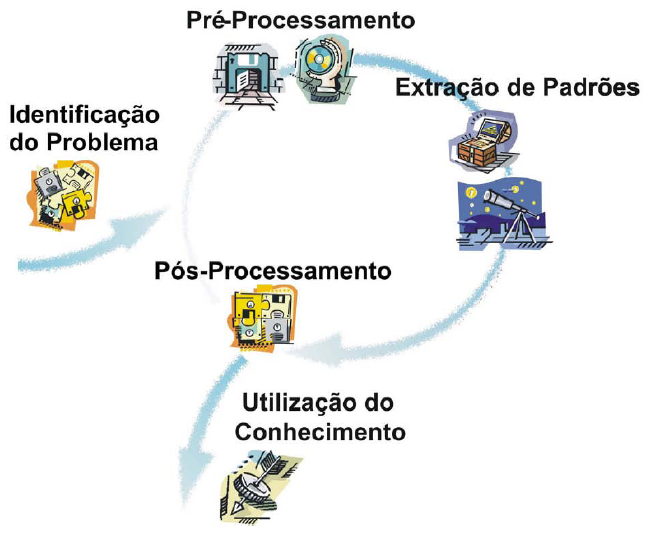
\includegraphics[scale=0.4]{./figuras/processo-kdd.png}
				\end{center}				
	            \label{fig:WM-KDD}
			\end{figure}		
	\end{frame}
	
	\begin{frame}
		\frametitle{\huge Web Mining}				
		 	\begin{figure}[htb]
				\begin{center}				
					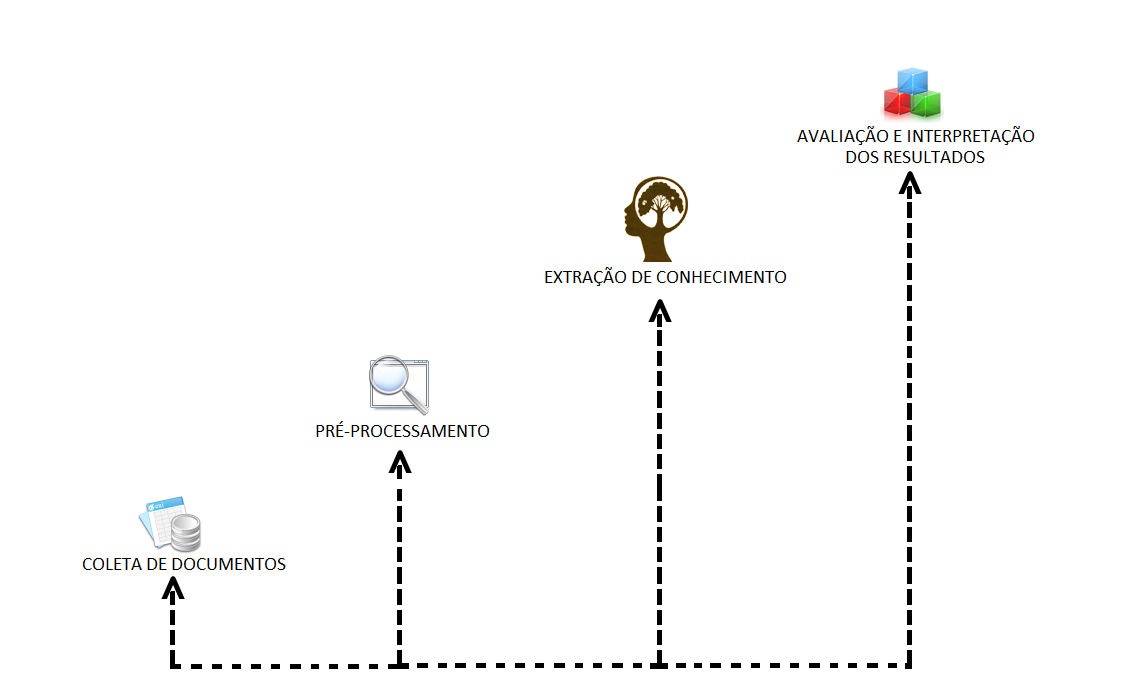
\includegraphics[scale=0.37]{./figuras/processo_webmining.png}
				\end{center}				
	            \label{fig:WM-KDD}
			\end{figure}		
	\end{frame}
	
	\begin{frame}
		\frametitle{\huge Web Mining}
		\framesubtitle{\Large Categorias}
		 	\begin{figure}[htb]
				\begin{center}				
					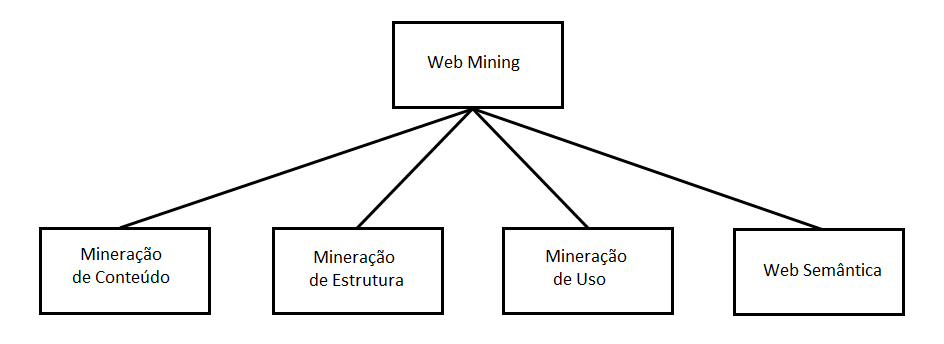
\includegraphics[scale=0.4]{./figuras/WB-taxonomia.png}
				\end{center}				
	            \label{fig:WM-KDD}
			\end{figure}		
	\end{frame}
	